\newpage
\section{Varianza pt.2}
Riprendiamo l'argomento della varianza che abbiamo gia visto nel capitolo 8.4 \ref{sec-varianza}
\\\\Data una variabile aleatoria $X \sim p_X(x)$, con $x \in \mathcal{X}$ e media $\mu_X = \mathbb{E}[X]$, definiamo i seguenti parametri fondamentali per descriverne la dispersione e la potenza.

\begin{itemize}
    \item \textbf{Il Valore Quadratico Medio} (Mean Square) di $X$:
    Rappresenta la media dei quadrati dei valori. mescola sia l'informazione su quanto sono grandi i valori (attorno alla media), sia quanto variano.
    
    \begin{equation}
    \boxed{X^2_{\text{rms}} = \mathbb{E}[X^2] = \sum_{x \in \mathcal{X}} x^2 p_X(x)}
    \end{equation}

    \item \textbf{Il Valore Efficace} (Root Mean Square, rms) di $X$:
    È semplicemente la radice quadrata del valore quadratico medio. è leggermente più alto della media, Se avessi avuto numeri negativi (es. -10 e +10), la media sarebbe stata 0, ma l'RMS sarebbe stato 10. L'RMS ignora il segno e misura la magnitudine complessiva.
    
    \begin{equation}
    X_{\text{rms}} = \sqrt{\mathbb{E}[X^2]} = \sqrt{\sum_{x \in \mathcal{X}} x^2 p_X(x)}
    \end{equation}

    \item \textbf{La Varianza} di $X$ ($\sigma_X^2$):
    Misura la dispersione attorno alla media. Partiamo dicendo che la Varianza é la media degli scarti al quadrato. Sviluppando il quadrato del binomio, ritroviamo la relazione fondamentale tra varianza, valore quadratico medio e media:

    \begin{equation}
    \begin{aligned}
    \sigma_X^2 &= \mathbb{E}\left[ (X - \mu_X)^2 \right] \\
    &= \sum_{x \in \mathcal{X}} (x^2 + \mu_X^2 - 2x\mu_X) p_X(x) \\
    &= \mathbb{E}[X^2] + \mu_X^2 - 2\mu_X\mathbb{E}[X] \\
    &= X^2_{\text{rms}} - \mu_X^2
    \end{aligned}
    \end{equation}
    
    Quindi: \textbf{Varianza = (Valore Quadratico Medio) - (Media al quadrato)}.

    \item \textbf{La Deviazione Standard} di $X$:
    È la radice quadrata della varianza e ha la stessa unità di misura della variabile $X$.
    
    \begin{equation}
    \sigma_X = \sqrt{\sigma_X^2} = \sqrt{\mathbb{E}[X^2] - \mu_X^2} = \sqrt{X^2_{\text{rms}} - \mu_X^2}
    \end{equation}
    Immagina che i tuoi dati siano vettori nello spazio. Come si calcola la lunghezza (distanza) in geometria? Con il Teorema di Pitagora: $c=\sqrt{a^2 + b^2}$.
    La Deviazione Standard (radice della varianza) è letteralmente la distanza euclidea dei tuoi dati dalla media, normalizzata.
\end{itemize}

\subsection{Esempio \#1: Variabile Binomiale $X \sim \mathcal{B}(N, p)$}
Analizziamo il calcolo della varianza per una distribuzione Binomiale, distinguendo il caso semplice ($N=1$) da quello generale.

\textbf{Caso $N=1$ (Bernoulli)}

In questo caso la variabile è una semplice Bernoulli: assume valore $1$ con probabilità $p$ e valore $0$ con probabilità $(1-p)$.

\begin{itemize}
    \item \textbf{Media:} $\mathbb{E}[X] = 1 \cdot p + 0 \cdot (1-p) = p$
    
    \item \textbf{Mean Square:}
    \[ \mathbb{E}[X^2] = 1^2 \cdot p + 0^2 \cdot (1-p) = p \]
    \textit{Nota: Poiché $1^2=1$ e $0^2=0$, per una Bernoulli $\mathbb{E}[X^2] = \mathbb{E}[X]$.}
    
    \item \textbf{Varianza:} Applicando la formula di König-Huygens:
    \[ \sigma_X^2 = \mathbb{E}[X^2] - (\mathbb{E}[X])^2 = p - p^2 = p(1-p) \]
    
    \item \textbf{Deviazione Standard:}
    \[ \sigma_X = \sqrt{p(1-p)} \]
\end{itemize}

\subsection{Caso Generale (Qualsiasi $N$)}

Vogliamo calcolare $\mathbb{E}[X^2]$ per ricavare la varianza. La definizione è:

\[ \mathbb{E}[X^2] = \sum_{k=0}^{N} k^2 p_X(k) = \sum_{k=0}^{N} k^2 \binom{N}{k} p^k (1-p)^{N-k} \]

\textit{(Nota: usiamo $q$ al posto di $1-p$ per brevità, ma è la stessa cosa).}

\paragraph{1. La prima riga: Semplificazione del $k^2$}
Poiché per $k=0$ il termine è nullo, la somma parte da $k=1$. Qui fa la semplificazione algebrica sui fattoriali:

\[
k \binom{N}{k} = k \frac{N!}{k!(N-k)!} = k \frac{N!}{k(k-1)!(N-k)!} = \frac{N!}{(k-1)!(N-k)!}
\]

Quindi la somma diventa:

\[
\sum_{k=1}^{N} k \frac{N!}{(k-1)!(N-k)!} p^k q^{N-k}
\]

\paragraph{2. Il "Trucco" della Derivata}
Qui avviene la "magia". Il libro estrae $Np$ e riscrive il resto sotto forma di derivata. Vediamo come ci arriva.

Guardiamo il termine $k p^k$.
In analisi sappiamo che la derivata di $p^k$ rispetto a $p$ è $k p^{k-1}$.
Se moltiplichiamo per $p$, otteniamo:

\[
p \cdot \frac{d}{dp}(p^k) = p \cdot k p^{k-1} = k p^k
\]

Quindi, ovunque vedi $k p^k$, puoi sostituirlo con l'operatore $p \frac{d}{dp}$ applicato a $p^k$.
quindi:
\begin{itemize}
    \item Prende l'espressione della riga precedente.
    \item Estrae una $N$ dal fattoriale $N!$ (che diventa $N \cdot (N-1)!$).
    \item Usa l'operatore derivata per far sparire la $k$ rimanente.
\end{itemize}

L'espressione diventa:

\[
\sum_{k=1}^{N} \frac{(N-1)!}{(k-1)!(N-k)!} p^k q^{N-k}
\]

Per capire quanto vale questa somma, facciamo un cambio di variabile: poniamo $j = k-1$. La somma diventa:

\[
\sum_{j=0}^{N-1} \binom{N-1}{j} p^{j+1} q^{(N-1)-j}
\]

Possiamo portare fuori un $p$ e riconosciamo lo sviluppo del binomio di Newton:

\[
p \cdot \underbrace{\sum_{j=0}^{N-1} \binom{N-1}{j} p^{j} q^{(N-1)-j}}_{(p+q)^{N-1}} = p(p+q)^{N-1}
\]

\paragraph{3. Calcolo della Derivata}
Ora il libro calcola la derivata rispetto a $p$ di quella quantità che abbiamo appena trovato: $p(p+q)^{N-1}$.
\\\textit{(Nota: in questa fase $q$ viene trattato come una costante fissa, la condizione $q=1-p$ si applica solo alla fine).}

Usiamo la regola del prodotto per derivare $p(p+q)^{N-1}$:
\begin{itemize}
    \item Derivata del primo ($p$) per il secondo non derivato: $1 \cdot (p+q)^{N-1}$
    \item Più il primo ($p$) per la derivata del secondo: $p \cdot (N-1)(p+q)^{N-2}$
\end{itemize}

Risultato della derivata:
\[
(p+q)^{N-1} + p(N-1)(p+q)^{N-2}
\]

\paragraph{4. Sostituzione finale}
Ora applichiamo la condizione $q = 1-p$, il che significa che $p+q = 1$.
L'espressione diventa semplicissima perché le potenze di 1 sono sempre 1:

\[
1^{N-1} + p(N-1)1^{N-2} = 1 + p(N-1)
\]

Moltiplichiamo per il fattore $Np$ che avevamo lasciato fuori dalla parentesi quadra all'inizio (come mostrato nel libro):

\[
\begin{aligned}
\mathbb{E}[X^2] &= Np [ 1 + p(N-1) ] \\
&= Np [ 1 + Np - p ] \\
&= Np + N^2 p^2 - Np^2
\end{aligned}
\]

Raggruppiamo i termini con $N$ singolo e quelli con $N^2$:

\[
= (Np - Np^2) + N^2 p^2 = Np(1-p) + N^2 p^2
\]

Ed ecco ottenuto esattamente il risultato del libro:

\begin{equation}
\mathbb{E}[X^2] = Np(1-p) + (Np)^2
\end{equation}

Dove $(Np)^2$ è il quadrato della media ($\mu_X^2$) e $Np(1-p)$ è la varianza.

\paragraph{Riepilogo}

Sostituendo il valore appena calcolato nella definizione generale di varianza ($\sigma_X^2 = \mathbb{E}[X^2] - \mu_X^2$), osserviamo che il termine $(Np)^2$ si elide.


\begin{equation}
\boxed{\mathbb{E}[X^2] = Np(1-p) + N^2 p^2} \quad \text{(Valore Quadratico Medio)}
\end{equation}

\begin{equation}
\boxed{\sigma_X^2 = Np(1-p)} \quad \text{(Varianza)}
\end{equation}

\begin{equation}
\boxed{\sigma_X = \sqrt{Np(1-p)}} \quad \text{(Deviazione Standard)}
\end{equation}

\textit{Nota: Spesso nei testi la varianza è indicata sinteticamente come $Npq$, ponendo $q = 1-p$.}

\subsection{Esempio \#2: Variabile Uniforme $X \sim \mathcal{U}(\{0, \dots, M-1\})$}

Consideriamo una variabile uniforme definita sull'insieme $\{0, \dots, M-1\}$, per la quale sappiamo che la media è $\mu_X = \mathbb{E}[X] = \frac{M-1}{2}$.

\paragraph{Calcolo del Mean Square (MS)}
Il valore quadratico medio si scrive come la media dei quadrati:

\[
X^2_{\text{rms}} = \frac{1}{M} \sum_{k=0}^{M-1} k^2 = \frac{1}{M} \sum_{k=1}^{M-1} k^2
\]

Per risolvere la sommatoria, sfruttiamo la nota identità per la somma dei primi $n$ quadrati:

\[
\sum_{i=1}^n i^2 = \frac{n(n+1)(2n+1)}{6}
\]

Applicando questa formula con $n = M-1$, il termine $(n+1)$ diventa $M$, che si semplifica con il fattore $\frac{1}{M}$ presente nella definizione del Mean Square. Otteniamo quindi:

\begin{equation}
X^2_{\text{rms}} = \frac{(M-1)(2M-1)}{6}
\end{equation}

\paragraph{Calcolo della Varianza}
Applicando la formula di König-Huygens ($\sigma^2 = \mathbb{E}[X^2] - \mu^2$):

\[
\sigma_X^2 = \frac{(M-1)(2M-1)}{6} - \left( \frac{M-1}{2} \right)^2
\]

\[
\sigma_X^2 = \frac{(M-1)(2M-1)}{6} - \frac{(M-1)^2}{4}
\]

Svolgendo i passaggi algebrici (minimo comune multiplo 12 e semplificazione dei termini), si giunge a un risultato fondamentale molto compatto:

\begin{equation}
\boxed{\sigma_X^2 = \frac{M^2 - 1}{12}}
\end{equation}

\paragraph{Riepilogo parametri}
Dai risultati precedenti ricaviamo immediatamente il valore efficace ($X_{\text{rms}}$) e la deviazione standard ($\sigma_X$):

\[
X_{\text{rms}} = \sqrt{\frac{(M-1)(2M-1)}{6}}
\]

\begin{equation}
\boxed{\sigma_X = \sqrt{\frac{M^2 - 1}{12}}}
\end{equation}

\subsection{Esempio \#3: Variabile di Poisson $X \sim \mathcal{P}(\lambda)$}

Consideriamo una variabile di Poisson con parametro $\lambda$. Ricordiamo che per questa distribuzione la media è $\mu_X = \mathbb{E}[X] = \lambda$.

\paragraph{Calcolo del Mean Square (MS)}
Partiamo dalla definizione di valore atteso del quadrato:
\[
X^2_{\text{rms}} = \sum_{k=0}^{\infty} k^2 \frac{\lambda^k e^{-\lambda}}{k!} = e^{-\lambda} \sum_{k=1}^{\infty} k^2 \frac{\lambda^k}{k!}
\]
\textit{(La somma parte da 1 perché il termine con $k=0$ è nullo).}

Semplifichiamo il fattoriale ($k/k! = 1/(k-1)!$):
\[
X^2_{\text{rms}} = e^{-\lambda} \sum_{k=1}^{\infty} k \frac{\lambda^k}{(k-1)!}
\]

Ora applichiamo il metodo della derivata. Notiamo che $k \lambda^k = \lambda \frac{d}{d\lambda}(\lambda^k)$. Possiamo quindi riscrivere l'espressione portando l'operatore di derivata fuori dalla sommatoria:

\[
X^2_{\text{rms}} = \lambda e^{-\lambda} \frac{d}{d\lambda} \left[ \sum_{k=1}^{\infty} \frac{\lambda^k}{(k-1)!} \right]
\]

\paragraph{Riconoscimento della Serie di Taylor}
Analizziamo il termine dentro la parentesi quadra. Dobbiamo ricondurci alla definizione di esponenziale ($e^\lambda = \sum \lambda^j/j!$).
\\Per farlo, portiamo fuori un $\lambda$ dalla somma in modo da allineare l'esponente con il fattoriale:

\[
\sum_{k=1}^{\infty} \frac{\lambda^k}{(k-1)!} = \lambda \sum_{k=1}^{\infty} \frac{\lambda^{k-1}}{(k-1)!}
\]

Ponendo il cambio di variabile $j = k-1$, la somma diventa esattamente lo sviluppo di Taylor di $e^\lambda$:

\[
\lambda \underbrace{\sum_{j=0}^{\infty} \frac{\lambda^j}{j!}}_{e^\lambda} = \lambda e^\lambda
\]

Sostituiamo questo risultato nella nostra espressione principale:

\[
X^2_{\text{rms}} = \lambda e^{-\lambda} \frac{d}{d\lambda} \left[ \lambda e^\lambda \right]
\]

\paragraph{Calcolo Finale}
Calcoliamo la derivata del prodotto $\lambda e^\lambda$ rispetto a $\lambda$:
\[
\frac{d}{d\lambda} (\lambda e^\lambda) = 1 \cdot e^\lambda + \lambda \cdot e^\lambda = e^\lambda(1 + \lambda)
\]

Sostituendo e semplificando ($e^{-\lambda} \cdot e^\lambda = 1$):
\[
X^2_{\text{rms}} = \lambda e^{-\lambda} [ e^\lambda(1 + \lambda) ] = \lambda (1 + \lambda) = \lambda + \lambda^2
\]

\paragraph{Riepilogo Risultati}
Ora possiamo calcolare la varianza sottraendo il quadrato della media ($\mu_X^2 = \lambda^2$).

\begin{equation}
\boxed{X^2_{\text{rms}} = \lambda + \lambda^2}
\end{equation}

\begin{equation}
\sigma_X^2 = (\lambda + \lambda^2) - \lambda^2 \implies \boxed{\sigma_X^2 = \lambda}
\end{equation}

\begin{equation}
\boxed{\sigma_X = \sqrt{\lambda}}
\end{equation}

\textbf{Nota Importante:} La distribuzione di Poisson gode di una proprietà unica e fondamentale: \textbf{la media e la varianza coincidono}.
\[ \mathbb{E}[X] = \text{Var}(X) = \lambda \] 

\section{Caratterizzazione Parziale e Disuguaglianze}

Supponiamo di non avere una caratterizzazione completa di una variabile aleatoria $X$. 
Non conosciamo cioè la sua PMF ($p_X(x)$) esatta. Tuttavia, spesso conosciamo alcuni parametri sintetici come la media $\mu_X$ e la varianza $\sigma_X^2$.

\subsection{L'importanza della non-negatività}
Se sappiamo che $X \subseteq [0, +\infty[$ (cioè la variabile è \textbf{non negativa}), la media $\mu_X$ ci fornisce un'informazione molto potente sul comportamento della variabile, anche se imprecisa.

\begin{itemize}
    \item \textbf{Numeri negativi vs positivi:} Se $X$ potesse essere negativa, una media $\mu=0$ non ci direbbe nulla sulla grandezza dei valori (potrebbe oscillare tra -1.000.000 e +1.000.000).
    \item \textbf{Vincolo dello zero:} Se invece $X \ge 0$ e la media è bassa, la variabile è \textbf{costretta} a stare vicino allo zero. Non possiamo avere valori giganti positivi senza avere valori negativi che li bilancino per tenere la media bassa.
\end{itemize}

In questo contesto, la media impone un \textbf{tetto massimo alla probabilità} che la variabile assuma valori molto alti.

\subsection{Disuguaglianza di Markov}

Questa disuguaglianza si applica a variabili aleatorie \textbf{non negative}. Esempi tipici sono grandezze fisiche (distanza, altezza, peso) o economiche (guadagno), mentre non si applica a temperature in gradi Celsius (che possono essere negative).

\begin{equation}
\boxed{P(X \ge t) \le \frac{\mathbb{E}[X]}{t}}
\end{equation}

Dove:
\begin{itemize}
    \item $\mathbb{E}[X]$ è il valore atteso (media).
    \item $t$ è una soglia (threshold) positiva ($t > 0$).
\end{itemize}

\subsubsection{Interpretazione Grafica e Dimostrazione Intuitiva}

Immaginiamo una distribuzione qualsiasi (non sappiamo com'è fatta, vedi Fig. 1). Vogliamo sapere qual è la probabilità che $X$ sia \textbf{ALMENO} $t$, sapendo solo dove si trova il baricentro (media).

\begin{center}
\begin{tikzpicture}
    \begin{axis}[
        width=10cm, height=5cm,
        axis lines=left,
        ticks=none,
        ymin=0, ymax=0.5,
        xmin=0, xmax=10,
        xlabel=$x$,
        ylabel=$f_X(x)$,
        clip=false
    ]
        % Distribuzione generica
        \addplot[thick, smooth, name path=curve] coordinates {
            (0,0) (1,0.1) (2,0.3) (3,0.35) (4,0.2) (5,0.1) (6,0.05) (10,0)
        };
        
        % Area sotto la curva (totale)
        \path[name path=axis] (axis cs:0,0) -- (axis cs:10,0);
        
        % Soglia t
        \draw[dashed, thick, red] (axis cs:4,0) -- (axis cs:4,0.4) node[above] {$t$};
        
        % Area evidenziata P(X >= t)
        \addplot[yellow!50, fill opacity=0.6] fill between[
            of=curve and axis,
            soft clip={domain=4:10}
        ];
        
        \node at (axis cs:5.5, 0.08) {$P(X \ge t)$};
        \node at (axis cs:2, 0.1) {$P(X < t)$};
        
        % Indicazione media (baricentro ipotetico)
        \draw[blue, thick, ->] (axis cs:3, -0.05) -- (axis cs:3, 0) node[below=5pt] {$\mathbb{E}[X]$};
    \end{axis}
\end{tikzpicture}
\\ \textit{Fig 1: Distribuzione generica con soglia $t$.}
\end{center}

Per dimostrarlo, usiamo la legge della probabilità totale (o partizione del valore atteso). Possiamo scrivere la media come somma pesata di due contributi: i valori minori di $t$ e i valori maggiori o uguali a $t$.

\begin{equation}
\mathbb{E}[X] = \underbrace{\mathbb{E}[X | X < t] \cdot P(X < t)}_{\text{Parte sinistra}} + \underbrace{\mathbb{E}[X | X \ge t] \cdot P(X \ge t)}_{\text{Parte destra}}
\end{equation}

Analizziamo i limiti inferiori di queste due parti:
1. Poiché $X \ge 0$, la media della parte sinistra è sicuramente $\ge 0$.
2. Nella parte destra, stiamo considerando solo valori $X \ge t$. Quindi, la media di questi valori deve essere per forza almeno $t$ ($\mathbb{E}[X | X \ge t] \ge t$).

Possiamo quindi scrivere la disuguaglianza:

\[
\mathbb{E}[X] \ge 0 \cdot P(X < t) + t \cdot P(X \ge t)
\]

\[
\mathbb{E}[X] \ge t \cdot P(X \ge t) \implies P(X \ge t) \le \frac{\mathbb{E}[X]}{t}
\]

\begin{center}
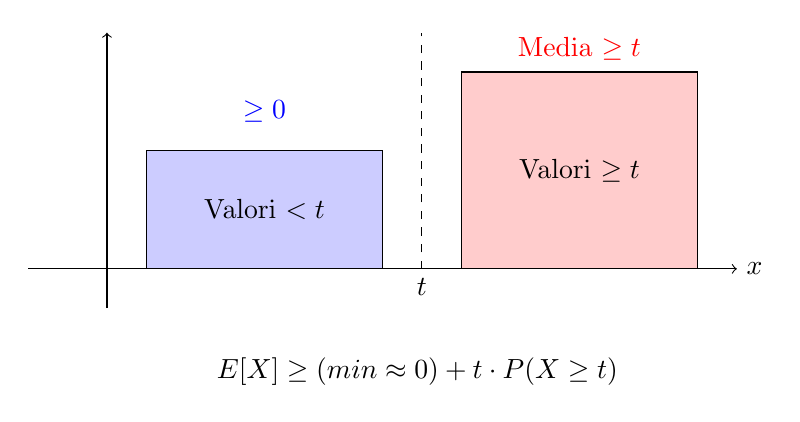
\begin{tikzpicture}
    % Rappresentazione a blocchi della dimostrazione
    \draw[->] (-1,0) -- (8,0) node[right] {$x$};
    \draw[->] (0,-0.5) -- (0,3);
    
    % Soglia t
    \draw[dashed] (4,0) node[below] {$t$} -- (4,3);
    
    % Blocco Sinistro (Minimizzato a 0)
    \draw[fill=blue!20] (0.5,0) rectangle (3.5, 1.5);
    \node at (2, 0.75) {Valori $< t$};
    \node[blue] at (2, 2) {$\ge 0$};
    
    % Blocco Destro (Minimizzato a t)
    \draw[fill=red!20] (4.5,0) rectangle (7.5, 2.5);
    \node at (6, 1.25) {Valori $\ge t$};
    \node[red] at (6, 2.8) {Media $\ge t$};
    
    % Equazione visiva
    \node[align=center, below] at (4, -1) {
    $\mathbb{E}[X] \ge (\text{min} \approx 0) + t \cdot P(X \ge t)$
    };
\end{tikzpicture}
\\ \textit{Fig 2: Intuizione della dimostrazione. Per avere massa a destra di $t$, devo "spendere" media.}
\end{center}

\paragraph{Perché funziona? (Ragionamento per assurdo)}
Supponiamo che la probabilità di superare la soglia sia più alta di quanto predetto da Markov:
\[ P(X \ge t) = \frac{\mathbb{E}[X]}{t} + \epsilon \]
Se spostiamo tutta la massa a sinistra sullo 0 (caso migliore per minimizzare) e tutta la massa a destra esattamente su $t$ (caso migliore), otterremmo comunque una media totale:
\[ \text{Nuova Media} = 0 + t \cdot \left(\frac{\mathbb{E}[X]}{t} + \epsilon\right) = \mathbb{E}[X] + t\cdot\epsilon \]
Che è strettamente maggiore della media vera $\mathbb{E}[X]$. Questo è un assurdo. 
\textit{"Non troppe cose possono essere sopra la media, oppure la media è più alta di quanto pensiamo."}

\paragraph{Esempio Reale: Lo Stipendio}
Ipotizziamo che $X$ sia lo stipendio di una persona a caso.
\begin{itemize}
    \item $\mathbb{E}[X] = 50.000\$$
    \item Vogliamo sapere la probabilità che uno guadagni $t = 100.000\$$.
\end{itemize}
Applicando Markov:
\[ P(X \ge 100k) \le \frac{50k}{100k} = \frac{1}{2} \]
Ovvero, non più di metà della popolazione può guadagnare più di 100k.
\\Se per assurdo ipotizzassimo che i 2/3 delle persone guadagnano 100k, allora il restante 1/3 dovrebbe guadagnare $-150k$ per mantenere la media a 50k, il che è impossibile (non si possono guadagnare soldi negativi).
\\In breve, la \textbf{disuguaglianza di Markov} afferma che:

Per una variabile aleatoria $X$ che assume solo valori \textbf{non negativi} ($X \ge 0$), la probabilità che $X$ superi una certa soglia positiva $t$ è limitata superiormente dal rapporto tra la sua media e quella soglia.

In termini più semplici:
\begin{quote}
    \textit{``È poco probabile che una variabile non negativa assuma valori molto più grandi della sua media.''}
\end{quote}

\newpage
\subsection{Disuguaglianza di Chebyshev}

Se conosciamo non solo la media, ma anche la \textbf{varianza}, abbiamo una caratterizzazione molto più precisa della variabile aleatoria. Supponiamo di conoscere la coppia $(\mu_X, \sigma_X^2)$.

La varianza ci dice quanto è probabile che $X$ sia lontana dalla media.
\begin{itemize}
    \item Se la varianza è piccola, la probabilità di allontanarsi è bassa.
    \item La probabilità che $X$ sia distante almeno $t$ dalla sua media non può essere troppo grande.
\end{itemize}

Matematicamente:
\begin{equation}
\boxed{P(|X - \mu_X| \ge t) \le \frac{\text{Var}(X)}{t^2}}
\end{equation}

\subsubsection{Interpretazione Grafica}
"The probability of being far from the mean can't be too big."
\\Visualizziamo cosa significa:

\begin{center}
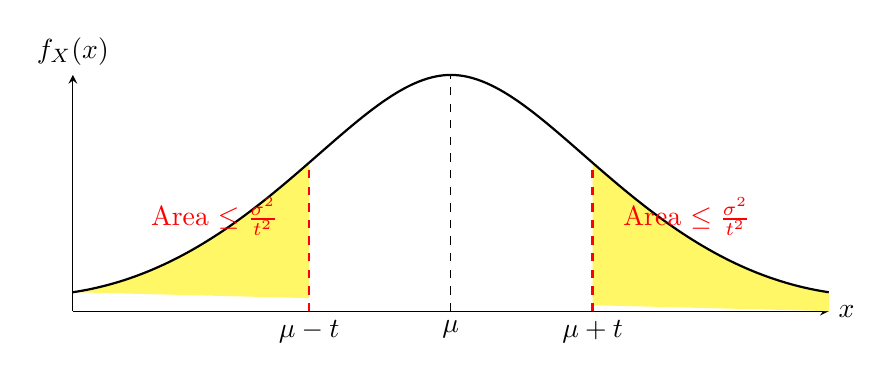
\begin{tikzpicture}[>=stealth, xscale=1.2, yscale=1.2]
    % Assi
    \draw[->] (0,0) -- (8,0) node[right] {$x$};
    \draw[->] (0,0) -- (0,2.5) node[above] {$f_X(x)$};

    % Curva a campana generica
    \def\bellcurve{(0,0.2) .. controls (2,0.5) and (3,2.5) .. (4,2.5) .. controls (5,2.5) and (6,0.5) .. (8,0.2)}

    % Riempimento Code (Aree Gialle)
    \begin{scope}
        % Coda Sinistra (x < mu - t) -> Diciamo mu=4, t=1.5 -> x < 2.5
        \clip (0,0) rectangle (2.5, 3);
        \fill[yellow!60] \bellcurve -- (8,0) -- cycle;
    \end{scope}
    \begin{scope}
        % Coda Destra (x > mu + t) -> x > 5.5
        \clip (5.5,0) rectangle (8, 3);
        \fill[yellow!60] \bellcurve -- (8,0) -- cycle;
    \end{scope}

    % Disegno contorno curva
    \draw[thick] \bellcurve;

    % Linee e etichette
    \draw[dashed] (4,0) -- (4,2.5); \node[below] at (4,0) {$\mu$};
    
    \draw[dashed, thick, red] (2.5,0) -- (2.5,1.5); \node[below] at (2.5,0) {$\mu - t$};
    \draw[dashed, thick, red] (5.5,0) -- (5.5,1.5); \node[below] at (5.5,0) {$\mu + t$};

    % Quote
    \node[align=center, red] at (1.5, 1) {Area $\le \frac{\sigma^2}{t^2}$};
    \node[align=center, red] at (6.5, 1) {Area $\le \frac{\sigma^2}{t^2}$};
\end{tikzpicture}
\end{center}

\subsubsection{Dimostrazione Algebrica (via Markov)}
Possiamo dimostrare Chebyshev in una riga usando Markov.
Definiamo una nuova variabile $Y = (X - \mu)^2$. Poiché è un quadrato, $Y$ è sicuramente \textbf{non negativa}.
Vogliamo calcolare la probabilità che la distanza sia $\ge t$, che equivale a dire che la distanza al quadrato è $\ge t^2$:

\[
P(|X - \mu| \ge t) = P((X - \mu)^2 \ge t^2)
\]

Applicando Markov alla variabile $(X-\mu)^2$ con soglia $t^2$:

\[
P((X - \mu)^2 \ge t^2) \le \frac{\mathbb{E}[(X - \mu)^2]}{t^2} = \frac{\text{Var}(X)}{t^2} \quad \text{C.V.D.}
\]

\subsubsection{Intuizione "Fisica": I Muri e il Collasso}
Proviamo a costruire un limite inferiore cercando di minimizzare la varianza mantenendo fissa la probabilità delle code.
Immaginiamo di costruire dei "muri" a distanza $t$ dalla media.

\begin{center}
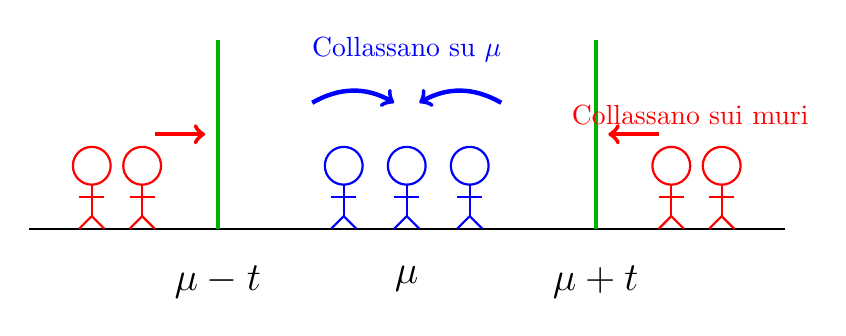
\begin{tikzpicture}[xscale=0.8, yscale=0.8]
    % Linea base
    \draw[thick] (-6,0) -- (6,0);
    
    % Muri
    \draw[ultra thick, green!70!black] (-3,0) -- (-3,3);
    \draw[ultra thick, green!70!black] (3,0) -- (3,3);
    
    % Labels asse
    \node[below=10pt] at (0,0) {\Large $\mu$};
    \node[below=10pt] at (-3,0) {\Large $\mu - t$};
    \node[below=10pt] at (3,0) {\Large $\mu + t$};

    % Omini Fuori (Stick figures)
    \foreach \x in {-5, -4.2} {
        \draw[thick, red] (\x, 1) circle (0.3); % testa
        \draw[thick, red] (\x, 0.7) -- (\x, 0.2); % corpo
        \draw[thick, red] (\x-0.2, 0.5) -- (\x+0.2, 0.5); % braccia
        \draw[thick, red] (\x, 0.2) -- (\x-0.2, 0); % gamba sx
        \draw[thick, red] (\x, 0.2) -- (\x+0.2, 0); % gamba dx
    }
    \foreach \x in {4.2, 5} {
        \draw[thick, red] (\x, 1) circle (0.3); 
        \draw[thick, red] (\x, 0.7) -- (\x, 0.2);
        \draw[thick, red] (\x-0.2, 0.5) -- (\x+0.2, 0.5);
        \draw[thick, red] (\x, 0.2) -- (\x-0.2, 0);
        \draw[thick, red] (\x, 0.2) -- (\x+0.2, 0);
    }

    % Omini Dentro (Stick figures blu)
    \foreach \x in {-1, 0, 1} {
        \draw[thick, blue] (\x, 1) circle (0.3); 
        \draw[thick, blue] (\x, 0.7) -- (\x, 0.2);
        \draw[thick, blue] (\x-0.2, 0.5) -- (\x+0.2, 0.5);
        \draw[thick, blue] (\x, 0.2) -- (\x-0.2, 0);
        \draw[thick, blue] (\x, 0.2) -- (\x+0.2, 0);
    }

    % Frecce di collasso
    \draw[->, ultra thick, blue] (1.5, 2) to[bend right] (0.2, 2);
    \draw[->, ultra thick, blue] (-1.5, 2) to[bend left] (-0.2, 2);
    \node[blue, above] at (0, 2.5) {Collassano su $\mu$};

    \draw[->, ultra thick, red] (-4, 1.5) -- (-3.2, 1.5);
    \draw[->, ultra thick, red] (4, 1.5) -- (3.2, 1.5);
    \node[red, above] at (4.5, 1.5) {Collassano sui muri};

\end{tikzpicture}
\end{center}

Per la legge della probabilità totale, dividiamo il valore atteso della varianza (che è $\mathbb{E}[(X-\mu)^2]$) in due parti: i valori che stanno "nel mezzo" e i valori che stanno "all'esterno".

\[
\text{Var}(X) = \underbrace{\mathbb{E}[(X-\mu)^2 \mid |X-\mu| < t] \cdot P(|X-\mu| < t)}_{\text{Parte Interna}} + \underbrace{\mathbb{E}[(X-\mu)^2 \mid |X-\mu| \ge t] \cdot P(|X-\mu| \ge t)}_{\text{Parte Esterna}}
\]

Ora applichiamo la logica del "collasso" per trovare il caso limite (minimo):
\begin{enumerate}
    \item \textbf{Parte Interna:} Tutti i valori nell'intervallo $\mu-t < X < \mu+t$ collassano esattamente su $\mu$.
    La loro distanza dalla media diventa $0$. Quindi questo termine contribuisce $\approx 0$.
    
    \item \textbf{Parte Esterna:} Tutti i valori che sono fuori (maggiori di $\mu+t$ o minori di $\mu-t$) collassano esattamente sui "muri" a distanza $t$.
    La loro distanza al quadrato è esattamente $t^2$.
\end{enumerate}

Sostituendo queste stime nella formula:

\[
\text{Var}(X) \ge 0 \cdot P(\dots) + t^2 \cdot P(|X-\mu| \ge t)
\]

Da cui otteniamo direttamente:
\[
\text{Var}(X) \ge t^2 \cdot P(|X-\mu| \ge t) \implies P(|X-\mu| \ge t) \le \frac{\text{Var}(X)}{t^2}
\]

\subsubsection{Dimostrazione Formale (Come nelle Slide)}
Spesso la disuguaglianza di Chebyshev viene presentata al contrario, ovvero chiedendosi: qual è la probabilità che il valore cada \textbf{vicino} alla media (dentro l'intervallo $[\mu - k\sigma, \mu + k\sigma]$)?

Poiché l'evento "stare dentro" è il complementare dell'evento "stare fuori", possiamo scrivere:

\[
P(\text{Dentro}) = 1 - P(\text{Fuori})
\]

Sapendo che $P(\text{Fuori}) \le \frac{1}{k^2}$, allora sottraendo questa quantità da 1 otteniamo:

\begin{equation}
\boxed{\mathbb{P}(\mu_X - k\sigma_X \le X \le \mu_X + k\sigma_X) \ge 1 - \frac{1}{k^2}}
\end{equation}
\begin{itemize}
    \item $k\sigma_X$: É il corrispettivo di t ma piu generico dove, $\sigma_X$ é l'unitá e k é il numero di "passi".
\end{itemize}


\textbf{Esempio numerico:}
Se scegliamo $k=2$ (due deviazioni standard):
\begin{itemize}
    \item La probabilità di essere fuori è $\le \frac{1}{4} = 25\%$.
    \item La probabilità di essere dentro l'intervallo è $\ge 1 - 25\% = 75\%$.
\end{itemize}
Quindi, per \textit{qualsiasi} distribuzione, almeno il 75\% dei dati cade entro 2 deviazioni standard dalla media.

Sia $Z$ una variabile aleatoria \textbf{non negativa} definita su un alfabeto discreto $\mathcal{Z} \subseteq [0, +\infty[$. Vogliamo valutare la probabilità che $Z$ superi una soglia $\delta \in \mathcal{Z}$.

\begin{equation}
\mathbb{P}(Z \ge \delta) = \sum_{z \ge \delta} p_Z(z) 
\stackrel{(a)}{\le} \sum_{z \ge \delta} \left(\frac{z}{\delta}\right)^2 p_Z(z) 
\stackrel{(b)}{\le} \sum_{z \in \mathcal{Z}} \left(\frac{z}{\delta}\right)^2 p_Z(z) 
\stackrel{(c)}{=} \frac{\mathbb{E}[Z^2]}{\delta^2}
\end{equation}

\textbf{Spiegazione dei passaggi:}
\begin{itemize}
    \item \textbf{(a)} Deriva dal fatto che stiamo sommando solo su $z \ge \delta$. In questa regione, la frazione $\frac{z}{\delta} \ge 1$, e quindi anche il suo quadrato $\left(\frac{z}{\delta}\right)^2 \ge 1$. Moltiplicare la probabilità per un numero $\ge 1$ può solo aumentare (o lasciare uguale) il valore della somma.
    \item \textbf{(b)} Estendiamo la sommatoria da un sottoinsieme ($z \ge \delta$) a tutto l'alfabeto $\mathcal{Z}$. Poiché stiamo aggiungendo termini non negativi (probabilità e quadrati sono sempre positivi), la somma totale aumenta sicuramente.
    \item \textbf{(c)} Portiamo fuori la costante $\frac{1}{\delta^2}$ e riconosciamo la definizione di valore quadratico medio: $\sum_{z \in \mathcal{Z}} z^2 p_Z(z) = \mathbb{E}[Z^2]$.
\end{itemize}

\paragraph{Applicazione a Chebyshev}
La disuguaglianza classica si ricava ponendo:
\[ Z = |X - \mu_X| \quad \text{e} \quad \delta = k\sigma_X \]
Notando che $Z \ge 0$ e che $\mathbb{E}[Z^2] = \mathbb{E}[|X-\mu_X|^2] = \text{Var}(X) = \sigma_X^2$, otteniamo:

\[
\mathbb{P}(|X - \mu_X| \ge k\sigma_X) \le \frac{\sigma_X^2}{(k\sigma_X)^2} = \frac{\sigma_X^2}{k^2 \sigma_X^2} = \frac{1}{k^2}
\]

\subsubsection{Interpretazione del rapporto $\mu / \sigma$}
Dalle slide emerge un'altra considerazione importante sulla "qualità" della variabile aleatoria.
Possiamo analizzare il comportamento di $X$ guardando il rapporto tra la sua media e la sua deviazione standard:

\begin{equation}
\text{Rapporto} = \frac{\mu_X}{\sigma_X}
\end{equation}

\begin{itemize}
    \item \textbf{Valori Elevati:} Indicano una PMF molto concentrata intorno alla media. L'errore relativo è basso. La variabile è "poco aleatoria" (quasi deterministica).
    \item \textbf{Valori Bassi:} Indicano un'elevata dispersione rispetto alla grandezza del valore medio. La variabile è molto aleatoria e "rumorosa".
\end{itemize}